\documentclass[12pt]{article}
\usepackage[utf8]{inputenc} 
\usepackage[T1]{fontenc}
\usepackage[spanish]{babel}
\usepackage{amsmath, amssymb}
\usepackage{graphicx}
\usepackage{hyperref}
\usepackage{enumitem}
\usepackage{setspace}
\usepackage{geometry}
\geometry{letterpaper, margin=1in}

\title{Simulación de Partido de Baloncesto: Revisión y Análisis Detallado}
\author{Josue Rolando Naranjo Sieiro}
\date{\today}

\begin{document}
\maketitle

\onehalfspacing

\section*{Resumen}
En este documento se presenta una revisión extensa y detallada del proyecto de simulación de un partido de baloncesto a través de eventos discretos. La simulación, implementada en Python, modela la dinámica del juego dividiéndolo en posesiones, en las que se consideran eventos como intentos de tiro, conversiones, tiros libres, faltas, turnovers, robos y rebotes. Los datos iniciales se tomaron de estadísticas de partidos de la NBA. Se detallan la definición del problema, el proceso de implementación, los experimentos y el análisis estadístico, concluyendo con las principales observaciones y sugerencias para futuras mejoras.

\newpage

\section{S1. Introducción}

\subsection{Breve Descripción del Proyecto}
El proyecto consiste en el desarrollo de un simulador de eventos discretos aplicado a un partido de baloncesto. La simulación se implementa en Python y modela el comportamiento de un encuentro deportivo dividiendo el juego en posesiones. En cada posesión se simulan eventos tales como intentos de tiro, conversiones, tiros libres, faltas, turnovers, robos y rebotes. Se utiliza un marco temporal compuesto por cuatro cuartos de 12 minutos cada uno, lo que permite investigar el impacto de diversas variables sobre el marcador final. Los datos iniciales utilizados se basaron en estadísticas reales de partidos de la NBA.

\subsection{Objetivos y Metas}
El objetivo principal es analizar y comprender cómo influyen diversos factores, principalmente la eficiencia ofensiva, la defensa y la dinámica de posesiones, en el resultado final de un partido de baloncesto. Las metas específicas del proyecto son:
\begin{itemize}
    \item \textbf{Determinar la influencia de la eficiencia en los tiros:} Incrementar la probabilidad de convertir tiros de 2 puntos de 50\% a 60\% y tiros de 3 puntos de 35\% a 40\% para evaluar su impacto en el marcador.
    \item \textbf{Estudiar el impacto de la defensa:} Reducir la probabilidad de turnovers (de 15\% a 10\%) y analizar cómo esto afecta el control del balón y el ritmo del juego.
    \item \textbf{Investigar la relación entre el número de posesiones y el marcador final:} Estimar el promedio de puntos por posesión (PPP) y determinar si el marcador es proporcional al número total de posesiones.
    \item  \textbf{Evaluar el impacto de la probabilidad de rebote ofensivo en el marcador final: } Comparar la situación baseline (con una probabilidad de rebote ofensivo del 30 \%) frente a una situación en la que se incrementa dicha probabilidad al 50 \%. 
    \item \textbf{Realizar un análisis estadístico exhaustivo:} Simular 1000 partidos para extraer promedios, realizar análisis de sensibilidad y validar la robustez del modelo.
\end{itemize}

\subsection{El Sistema Específico a Simular y las Variables de Interés}
El sistema a simular es un partido de baloncesto, considerado como una sucesión de posesiones discretas. Cada posesión se modela como una unidad en la que se produce un intento de tiro que puede incluir la ocurrencia de foul, tiro libre, rebote ofensivo o defensivo y, en caso de error, un turnover. Las variables de interés del sistema son:
\begin{itemize}
    \item \textbf{Tiempo de juego:} 4 cuartos de 12 minutos cada uno (720 segundos por cuarto).
    \item \textbf{Número de posesiones:} Aproximadamente entre 90 y 120 por equipo por partido, según la duración de cada posesión.
    \item \textbf{Eficiencia de tiro:} Porcentajes de acierto para tiros de 2 puntos y 3 puntos (inicialmente 50\% y 35\%, modificados a 60\% y 40\%) y para tiros libres (80\% en promedio).
    \item \textbf{Eventos defensivos:} Probabilidades de turnovers, de robos (66\% de los turnovers se convierten en robos) y la distribución de rebotes (ofensivos y defensivos).
    \item \textbf{Otros eventos:} La ocurrencia de fouls y la derivación de tiros libres, que pueden ocurrir en forma de “and one” o tiros libres equivalentes en caso de fallo.
\end{itemize}

\subsection{Variables que Describen el Problema}
Las principales variables que describen el problema son:
\begin{itemize}
    \item El número total de posesiones por partido.
    \item Los puntos por posesión (PPP), que relacionan la eficiencia ofensiva con el marcador final.
    \item Las tasas de conversión de tiros de 2 puntos, tiros de 3 puntos y tiros libres.
    \item Los errores ofensivos (turnovers) y las oportunidades defensivas (robos).
    \item La distribución de rebotes entre ofensivos y defensivos, que influye en el número efectivo de posesiones.
\end{itemize}

\newpage

\section{S2. Detalles de Implementación}

\subsection{Definición del Problema y los Objetivos}
El primer paso consistió en definir claramente el problema: simular un partido de baloncesto para entender cómo afectan la eficiencia de tiro, la defensa y la dinámica de posesiones el marcador final. Se establecieron objetivos SMART:
\begin{itemize}
    \item \textbf{Específico:} Evaluar la relación entre el número de posesiones y el marcador, y cómo varían estos indicadores al modificar probabilidades clave.
    \item \textbf{Medible:} Se obtienen estadísticas (puntos promedio, intentos de tiro, turnovers, etc.) mediante la simulación de 1000 partidos.
    \item \textbf{Alcanzable:} Utilizando parámetros basados en datos reales de la NBA y supuestos empíricos.
    \item \textbf{Relevante:} Facilita la toma de decisiones informadas sobre la influencia de factores clave en el rendimiento de un equipo.
    \item \textbf{Plazo:} Establecido dentro del marco académico del proyecto.
\end{itemize}
Se delimitaron las fronteras del sistema modelando únicamente las posesiones y los eventos clave a nivel de equipo, excluyendo detalles individuales y estrategias complejas.

\subsection{Identificación y Recolección de Datos}
Se determinó la información necesaria para construir el modelo:
\begin{itemize}
    \item \textbf{Datos de juego:} Duración de 4 cuartos de 12 minutos cada uno y el número aproximado de posesiones por equipo.
    \item \textbf{Estadísticas ofensivas:} Porcentajes de acierto para tiros de 2 y 3 puntos (inicialmente 50\% y 35\%, modificados a 60\% y 40\%), y porcentaje de acierto en tiros libres (80\%).
    \item \textbf{Datos defensivos:} Número de turnovers (modificado de 15\% a 10\%), robos (66\% de los turnovers se registran como robos) y rebotes.
    \item \textbf{Fuentes:} Los datos iniciales provienen de estadísticas de partidos de la NBA y de fuentes académicas, ajustados mediante modelos probabilísticos (por ejemplo, distribuciones Bernoulli).
\end{itemize}

\subsection{Construcción del Modelo Conceptual}
Se desarrolló un modelo conceptual con un diagrama de flujo que ilustra:
\begin{itemize}
    \item El inicio del partido, dividido en 4 cuartos de 720 segundos cada uno.
    \item La asignación aleatoria de posesiones, con cada posesión modelada mediante un intento de tiro que incluye posibles resultados (acierto, fallo, foul) y la ocurrencia de turnovers o rebotes.
    \item La actualización del marcador y la transferencia de la posesión.
\end{itemize}
Se documentaron todas las suposiciones: la independencia de cada posesión y el uso de probabilidades fijas para simular cada evento (foul, tiro, rebote, etc.).

\subsection{Traducción del Modelo a Código/Software}
El modelo se implementó en Python, siguiendo estos pasos:
\begin{itemize}
    \item Definir la clase \texttt{Team} para almacenar estadísticas (puntuación, intentos, aciertos, turnovers, robos, rebotes).
    \item Desarrollar funciones específicas como \texttt{attempt\_shot}, \texttt{simulate\_possession} y \texttt{simulate\_quarter} para reproducir la lógica de cada posesión.
    \item Organizar el código de forma modular, facilitando su mantenimiento y extensión.
\end{itemize}

\subsection{Verificación y Validación}
\begin{itemize}
    \item \textbf{Verificación:} Se realizaron pruebas unitarias en funciones individuales para asegurar su correcto comportamiento.
    \item \textbf{Validación:} Se compararon los resultados simulados (puntos, intentos, turnovers) con estadísticas empíricas de la NBA y se evaluó la consistencia de los parámetros de regresión lineal (PPP).
\end{itemize}

\subsection{Experimentación y Análisis}
\begin{itemize}
    \item Se simularon 1000 partidos para obtener promedios robustos.
    \item Se realizaron experimentos variando parámetros como la eficiencia de tiro y la tasa de turnovers.
    \item Se efectuó un análisis de regresión para determinar la relación entre el número total de posesiones y el marcador final, evaluando el PPP y el coeficiente de correlación.
\end{itemize}

\subsection{Documentación y Elaboración de Informes}
\begin{itemize}
    \item Se elaboró un informe técnico que documenta desde la definición del problema hasta el análisis estadístico.
    \item El código fuente se acompañó de comentarios detallados para facilitar futuras revisiones.
    \item Se generaron gráficos y tablas que respaldan los hallazgos obtenidos durante la simulación.
\end{itemize}

\newpage

\section{S3. Resultados y Experimentos}

\subsection{Hallazgos de la Simulación}
\begin{itemize}
    \item \textbf{Eficiencia Ofensiva y Marcador:} El aumento de las probabilidades de acierto (60\% para tiros de 2 puntos y 40\% para tiros de 3 puntos) se tradujo en un incremento notable de la puntuación final en comparación con parámetros iniciales más conservadores.
    \item \textbf{Impacto de los Turnovers:} Reducir la probabilidad de turnovers de 15\% a 10\% produjo una disminución en el número de errores (aproximadamente 8.6--8.8 turnovers por partido) y un ajuste en el ritmo del juego, resultando en un marcador combinado promedio de alrededor de 112 puntos por equipo.
    \item \textbf{Relación entre Posesiones y Marcador Final:} El análisis de regresión lineal entre el número total de posesiones y el marcador final combinado generó la siguiente ecuación:
    \[
    \text{Marcador Total} = 1.23 \times \text{Posesiones} + 34.18,
    \]
    con un coeficiente de correlación (R) de 0.30.
\end{itemize}

\subsection{Interpretación de los Resultados}
\begin{itemize}
    \item La eficiencia ofensiva es crucial: incrementar la tasa de conversión en tiros se traduce en un mayor puntaje.
    \item La reducción de turnovers mejora el control del balón y reduce las oportunidades de contraataque, lo cual influye en el ritmo del juego y en el marcador final.
    \item Aunque se observa una relación positiva entre el número de posesiones y el marcador final (con una pendiente equivalente al PPP), el coeficiente de correlación moderado (R=0.30) indica que otros factores (fouls, rebotes, tiros libres, etc.) también inciden significativamente en el resultado.
\end{itemize}

\subsection{Hipótesis Extraídas de los Resultados}
\begin{enumerate}
    \item La eficiencia ofensiva, medida en puntos por posesión, es directamente proporcional al marcador final, manteniéndose constante el número de posesiones.
    \item Una reducción en la tasa de turnovers mejora el control del balón y reduce el ritmo del juego, afectando de forma indirecta el marcador.
    \item Aunque existe una relación positiva entre el número total de posesiones y el marcador final, la variabilidad introducida por otros eventos (fouls, rebotes y tiros libres) explica la moderada correlación observada.
\end{enumerate}

\subsection{Experimento: Impacto de la Probabilidad de Rebote Ofensivo}
Para evaluar el impacto de la probabilidad de rebote ofensivo en el marcador final, se realizaron dos experimentos:
\begin{itemize}
    \item \textbf{Escenario Baseline:} Se utilizó una probabilidad de rebote ofensivo del 30\%.
    \item \textbf{Escenario Mejorado:} Se incrementó la probabilidad de rebote ofensivo al 50\%.
\end{itemize}
La simulación de 1000 partidos en ambos escenarios arrojó que:
\begin{itemize}
    \item El marcador total promedio en el escenario baseline fue de 211.92 puntos.
    \item El marcador total promedio en el escenario mejorado fue de 230.07 puntos.
\end{itemize}
La prueba t de muestras independientes arrojó una t-statistic de 24.521 y un p-value muy bajo (p-value = 0.000), lo que indica que la diferencia es estadísticamente significativa. Estos resultados demuestran que incrementar la probabilidad de rebote ofensivo incrementa el marcador final, ya que se generan más oportunidades de tiro en la misma posesión.

A continuación se muestra la figura que ilustra este experimento:

\begin{figure}[h]
    \centering
    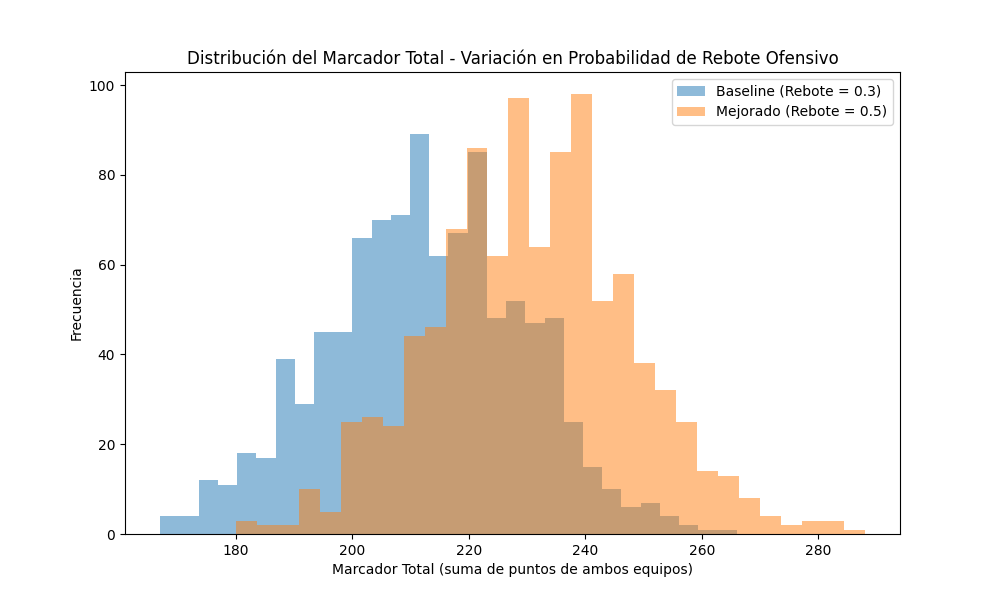
\includegraphics[width=\textwidth]{Figure_3.png}
    \caption{Impacto de la Probabilidad de Rebote Ofensivo: Comparación entre un escenario con rebote ofensivo del 30\% y otro con 50\%.}
    \label{fig:rebotes}
\end{figure}

\subsection{Experimentos Realizados para Validar las Hipótesis}
\begin{itemize}
    \item Se realizaron simulaciones variando las probabilidades de acierto en tiros de 2 y 3 puntos, observándose incrementos en el marcador final.
    \item La modificación de la tasa de turnovers (de 15\% a 10\%) redujo el número de errores, lo cual afectó el ritmo del juego y la distribución de rebotes.
    \item Se efectuó un análisis de regresión lineal para relacionar el número total de posesiones con el marcador final, obteniéndose un PPP promedio y una correlación moderada.
    \item Además, el experimento que varía la probabilidad de rebote ofensivo (de 30\% a 50\%) mostró un incremento significativo en el marcador final, validado mediante un test t.
\end{itemize}

\subsection{Necesidad de Análisis Estadístico}
El análisis estadístico resulta indispensable para:
\begin{itemize}
    \item Cuantificar el promedio de puntos por posesión mediante la regresión lineal.
    \item Validar la consistencia del modelo comparándolo con estadísticas reales de la NBA.
    \item Realizar un análisis de sensibilidad que determine cómo varían el marcador y otras métricas ante cambios en parámetros críticos.
\end{itemize}

\subsection{Análisis de Parada de la Simulación}
El modelo establece un límite temporal de 720 segundos por cuarto, lo cual garantiza que cada cuarto y, en consecuencia, cada partido, se detenga de manera realista. Esta metodología permite contabilizar de forma adecuada el número de posesiones y respetar las restricciones temporales propias de un encuentro real.

\newpage

\section{S4. Conclusiones}
El proyecto de simulación del partido de baloncesto ha permitido desarrollar un modelo de eventos discretos que refleja de manera aproximada la dinámica de un encuentro deportivo. Entre las conclusiones más importantes se destacan:
\begin{enumerate}
    \item \textbf{Importancia de la Eficiencia Ofensiva:} El incremento en la probabilidad de acierto en tiros (60\% para tiros de 2 puntos y 40\% para tiros de 3 puntos) ha demostrado ser determinante para aumentar la puntuación final.
    \item \textbf{Impacto del Control del Balón:} La reducción de la tasa de turnovers (de 15\% a 10\%) mejora el manejo del balón y reduce los errores ofensivos, modificando el ritmo del juego y afectando el marcador final.
    \item \textbf{Relación Posesiones-Marcador:} El análisis de regresión lineal evidencia que, en promedio, cada posesión adicional aporta 1.23 puntos; sin embargo, la correlación moderada (R=0.30) sugiere que otros factores (fouls, rebotes, tiros libres, etc.) también inciden fuertemente en el resultado.
    \item \textbf{Impacto de la Probabilidad de Rebote Ofensivo:} El nuevo experimento demuestra que aumentar la probabilidad de rebote ofensivo (de 30\% a 50\%) incrementa significativamente el marcador final, lo que confirma la hipótesis de que mayor recuperación de rebotes en ataque se traduce en más oportunidades de anotar.
    \item \textbf{Robustez del Modelo y Perspectivas Futuras:} El modelo se muestra robusto y sirve como base para futuras mejoras, tales como la incorporación de asimetrías entre equipos, efectos de racha (momentum) y análisis multivariable que incluya otros indicadores (por ejemplo, la duración promedio de posesión). Esto permitirá una comprensión más completa del comportamiento del juego.
\end{enumerate}
En definitiva, la simulación proporciona una herramienta cuantitativa para analizar cómo la interacción de variables clave---como la eficiencia en tiros, los turnovers, el número total de posesiones y la capacidad de recuperar rebotes ofensivos---determina el resultado final de un partido de baloncesto. El enfoque metodológico adoptado, desde la definición del problema hasta el análisis estadístico, sienta las bases para futuras investigaciones en simulación deportiva y la toma de decisiones estratégicas.

\end{document}
